\chapter{Потенциал}

\section{Теорема о циркуляции поля \textbf{E}}
    
    \begin{theorem}
        Циркуляция электростатического поля \( \vec{E} \) равна нулю, то есть
        \begin{equation}
            \oint\limits_C \vec{E}\cdot\dd\vec{l} = 0. \label{eq3:1}
        \end{equation}
    \end{theorem}
    
    \begin{proof}
        Есть два способа доказательства:
        \begin{enumerate}
            \item Вычислим работу поля
                \[
                    \vec{E} = \frac{q}{4\pi\varepsilon_0 r^2}
                \]
                одиночного точечного заряда \( q \) от точки 1 до точки 2:
                
                \[ 
                    A_{1\to2} = \int\limits_{1}^{2} \vec{E}\cdot\dd\vec{l} =
                    \int\limits_{1}^{2} E \dd l \cos\alpha =
                    \int\limits_{1}^{2} \frac{q}{4\pi\varepsilon_0 r^2}\dd r =
                    \frac{q}{4\pi\varepsilon_0}\left(\frac{1}{r_1} -
                    \frac{1}{r_2}\right)
                \]
            
            \item (см. Тензорный анализ 6.1.2 - 2)
                Так как 
                \[
                    \vec{E} = \frac{q}{4\pi\varepsilon_0}\cdot
                    \frac{\vec{r}}{r^3},
                \] 
                то
                \begin{align*}
                    & \int\limits_1^2 \vec{E}\cdot\dd\vec{l} =
                    \frac{q}{4\pi\varepsilon_0} \int\limits_1^2
                    \frac{xdx + ydy + zdz}{r^3} =
                    \frac{q}{4\pi\varepsilon_0}\cdot\frac{1}{2}\int\limits_1^2
                    \frac{\dd(x^2+y^2+z^2)}{r^3} = \\ = &
                    \frac{q}{4\pi\varepsilon_0} \int\limits_1^2 
                    \frac{r}{r^3}\dd r =
                    \frac{q}{4\pi\varepsilon_0}\left(\frac{1}{r_1} - 
                    \frac{1}{r_2}\right).
                \end{align*}
        \end{enumerate}
        Видно, что результат не зависит от формы пути, а только от 
        координат начальной и конечной точек.
        
        В частности, если \( \vec{r}_1 = \vec{r}_2 \), то есть кривая 
        образует замкнутый контур \( C \), то
        \[
            \oint\limits_C \vec{E}\cdot\dd\vec{l} = 0.
        \]
        
        Если поле \( \vec{E} \) образовано группой зарядов, то, в силу 
        принципа суперпозиции,
        \[ 
            \vec{E} = \sum\limits_k \vec{E}_{k},
        \]
        \[
            \oint\limits_C \vec{E}\cdot\dd\vec{l} =
            \sum\limits_k \oint\limits_{C_k}
            \vec{E}_{k}\cdot\dd\vec{l} = 0.
        \]
        
        Таким образом, для \( \vec{E} \):
        \[
            \oint\limits_C \vec{E}\cdot\dd\vec{l} = 0.
        \]
        
    \end{proof}
    
    \begin{definition}
        Всякое поле, циркуляция по контуру которого равна 0, является     
        \textbf{потенциальным}.
    \end{definition}
    
    Таким образом, \( \vec{E} \) -- потенциальное. По теореме Стокса:
    \[
        \oint\limits_C \vec{E}\cdot\dd\vec{l} = \iint\limits_S 
        \rot\vec{E}\cdot\dd\vec{S} \Rightarrow \rot\vec{E} = 0
        \text{, т.е. поле \( \vec{E} \) -- безвихревое}
    \]
    
    Получаем основные уравнения электростатики, которые вы можете видеть в 
    таблице \ref{fund_eq_e}. 
    
    \begin{table}[ht]
        \center
        \caption{Основные уравнения электростатики} \label{fund_eq_e}
        \begin{tabular}[ht]{|c|c|c|c|} \hline
            Название & \( \int \)-форма & \( \dd \)-форма & Смысл \\ \hline
            %------------------------------------------------------------
            & & & \\ % dirty hack for vertical space
            Теорема Гаусса & \( \oiint\limits_S\vec{E}\cdot\dd\vec{S}    
            =\frac{q_{S}}{\Ezero} \) & \( \div\vec{E}=\frac{\rho}{\Ezero} \)
            & поле \( \vec{E} \) рождается в источниках (\( \rho \)) \\
            %------------------------------------------------------------
            Теорема о циркуляции & \( \int\limits_C\vec{E}\cdot\dd\vec{l}=0 \) 
            & \( \rot\vec{E}=0 \) & поле \( \vec{E} \) - потенциально \\ \hline
            %------------------------------------------------------------
        \end{tabular}
    \end{table}
    
    \begin{remark}
        Линии поля \( \vec{E} \) \textit{не могут} быть замкнутыми, так как 
        выбрав контур по этой линии, то есть 
        \( \dd\vec{l} \uparrow\uparrow \vec{E} \) в каждой точке, получим 
        \[
            \oint\limits_C \vec{E}\cdot\dd\vec{l} = \oint\limits_{C} E\dd l > 0,
        \]
        что противоречит (\ref{eq3:1}).
    \end{remark}
    
\section{Потенциал и разность потенциалов}
    
    Так как \( \vec{E} \) -- потенциально, то его работа от точки 1 до точки 2:
    \[
        A_{1\to2} = \int\limits_1^2 \vec{E}\cdot\dd\vec{l} =
        \varphi_1 - \varphi_2,
    \]
    где \( \varphi_1,\ \varphi_2 \) -- функции координат точек 1 и 2 
    соответственно, и не зависит от формы кривой \( 1 \rightarrow 2 \).
    
    Чтобы определить \( \varphi \) поля \( \vec{E} \) как однозначную функцию 
    координат точки: \( \varphi = \varphi(x, y, z) \), обычно делают так:
    \begin{itemize}
        \item фиксируют точку 2 в качестве базовой точки \(M_0(x_0, y_0, z_0)\);
        \item полагают \( \varphi(M_0) = 0 \);
        \item точку 1 берут в качестве \( M(x, y, z) \), в которой и определяют 
            потенциал.
    \end{itemize}
    
    Если заряд (или группа зарядов) уединён, то \( M_0 \) - лежит на 
    бесконечности и \( \varphi(M_0) = 0 \). Если заряд распределён по 
    бесконечному объекту, то ни в нуле, ни в бесконечности
    \( \varphi(M_0) \ne 0 \).
    
    Итак, для ограниченных объектов поток их поля:
    \[
        \varphi(M) = \int\limits_M^{\infty} \vec{E}\cdot\dd\vec{l}
        \text{\ по любому пути}.
    \]
    
    Последнее уравнение -- это работа по перемещению заряда из данной точки в 
    бесконечность.
    
    \begin{definition}
        Выражение
        \[
            \Delta\varphi = \varphi_2 - \varphi_1 = \int\limits_1^2 
            \vec{E}\cdot\dd\vec{l}
        \]
        называется \textbf{разностью потенциалов} между точками 1 и 2 в поле
        \( \vec{E} \), а функция \( \varphi \) -- \textbf{потенциалом}.
    \end{definition}
    
    Размерность:
    \[
        [\varphi] = [\Delta\varphi] = \text{В},
    \]
    \[
        E = \frac{\varphi}{l} = \frac{\text{В}}{\text{м}}.
    \]
    
    Из принципа суперпозиции для \( \vec{E} \) следует свойство аддитивности 
    потенциалов: потенциал группы зарядов равен алгебраической сумме 
    потенциалов отдельных зарядов:
    \[
        \varphi = \sum\limits_k \pm \varphi_{k}.
    \]
    
    Итак, потенциал
    \begin{equation}
        \label{eq3:2}
        \varphi_{M} = \int\limits_M^{\infty} \vec{E}\cdot\dd\vec{l}
    \end{equation}
    Домножим (\ref{eq3:2}) на \( q \), получим    
    \[
        q\varphi_{M} = \int\limits_M^{\infty} q\vec{E}\cdot\dd\vec{l};
    \]
    а так как по определению \( \vec{E} = \frac{\vec{F}}{q} \), то
    \[
        q\varphi_{M} = \int\limits_M^{\infty} \vec{F}\cdot\dd\vec{l} =
        A_{M \rightarrow \infty}
    \]
    есть работа поля \( \vec{E} \) по переносу заряда \( q \) от точки \( M \)
    на \( \infty \).

    А так как \( A_{M \rightarrow \infty} \) в потенциальном поле равна 
    потенциальной энергии частицы \( W \) в точке \( M \), то 
    \[
        \varphi_{M} = \frac{W}{q} \left(\frac{\text{Дж}}{\text{Кл}} =
        \text{В}\right)
    \]
    
    Таким образом, потенциал точки \( M \) равен 1В, если заряд \( q = 1\)Кл 
    обладает в точке \( M \) энергией 1Дж.
    
    \begin{remark}
        В физике используется малая внесистемная единица энергии электрон-вольт 
        (эВ).
        
        По определению, 1эВ -- энергия заряда
        \( q = 1e = 1,6 \cdot 10^{-19} \)~Кл в точке поля
        \( \varphi = 1 \)~В (или ускоренного таким потенциалом).
        
        \[
            W = 1\text{эВ} = 1,6 \cdot 10^{-19}\text{Кл\( \cdot \)В} =
            1,6 \cdot 10^{-19}\text{ Дж}.
        \]
    \end{remark}
    
\section{Вычисление потенциалов}

    \begin{example}
        Найти потенциал точечного заряда \( q \).
    \end{example}
    
    \begin{solution}
        Так как путь можно выбирать любой, то пойдём в \( \infty \) по \( 
        \vec{r} \): \( \dd\vec{l} = \dd\vec{r} \).
        \[
            \vec{E} = \frac{q}{4\pi\varepsilon_0 r^3} \vec{r},
        \]
        \[
            \varphi(r) = \int\limits_r^{\infty} E(r)\dd r = 
            \frac{q}{4\pi\varepsilon_0} \int\limits_r^{\infty}
            \frac{1}{r^2}\dd r = \frac{q}{4\pi\epsilon_0 r}.
        \]
    \end{solution}
    
    \begin{example}
        Определить распределение потенциала поля заряженной сферы радиуса
        \( R \), несущей заряд \( q \).
    \end{example}
    
    \begin{figure}[!b]
        \center
        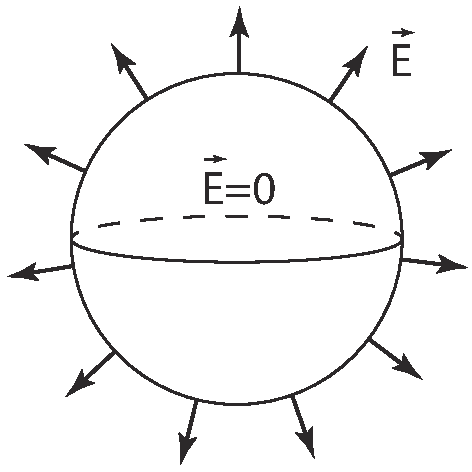
\includegraphics[width=.47\textwidth]{lec03/sphere.pdf}
        \hfill
        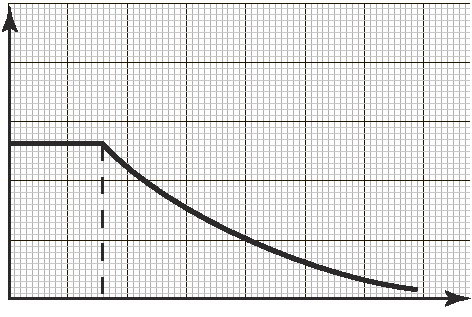
\includegraphics[width=0.47\textwidth]{lec03/sphere_plot.pdf}
        \parbox[t]{.47\textwidth}{\caption{Заряженная сфера}\label{3:sphere}}
        \hfill
        \parbox[t]{.47\textwidth}{\caption{Потенциал заряженной сферы}
        \label{3:sphere_plot}}
    \end{figure}
    
    \begin{solution}
        Сфера представлена на рисунке~\ref{3:sphere}. Как и в прошлый раз, 
        разобъём задачу на 2 подзадачи:
    \begin{enumerate}
        \item \( r > R \):        
            
            Так как поле сферы при \( r > R \)
            \[
                E = \frac{q}{4\pi\varepsilon_0 r^2},
            \]
            а работа потенциального поля не зависит от формы пути, то уходим в 
            бесконечность по радиусу:
            \[
                \varphi(r) = \int\limits_r^{\infty} E(r)\dd r = 
                \frac{q}{4\pi\varepsilon_0 r}
            \]
        \item \( r < R \):
        
            Идём по двум этапам:
            \[
                \varphi(r) = \int\limits_r^R E_{\textit{внутр}}(r)\dd r + 
                \int\limits_R^{\infty} E_{\textit{внеш}}(r)\dd r = 
                \frac{q}{4\pi\varepsilon_0 R} = \const
            \]
            График распределения потенциала сферы \( \varphi (r) \) представлен 
            на рисунке~\ref{3:sphere_plot}.
    \end{enumerate}
    \end{solution}
    
    \begin{example} % picture here or somewhere
        Вычислить разность потенциалов между точками 1 и 2 в  поле нити, 
        заряженной \( e \) с погонной плотностью \( \gamma \).
    \end{example}
    
    \begin{solution}
    Так как \( \Delta\varphi_{1 \to 2} \) не зависит от формы пути, то выбираем 
    путь так: \( 1 \to 2 = 1 \to 1’ + 1’ \to 2 \).
    \[
        \Delta\varphi_{1 \to 2} = \int\limits_1^{1’} \vec{E}\cdot\dd\vec{l} + 
        \int\limits_{1’}^2 \vec{E}\cdot\dd\vec{l}
    \]
    
    Так как \( \vec{E} \uparrow\uparrow \dd\vec{l}_{1 \to 1’} \) и
    \( \vec{E} \perp \dd\vec{l}_{1’ \to 2} \), то
    \[
        \Delta\varphi_{1 \to 2} = \int\limits_{r_1}^{r_2} 
        \frac{\gamma}{2\pi\varepsilon_0 r}\dd r = 
        \frac{\gamma}{2\pi\varepsilon_0}\ln{\frac{r_2}{r_1}}
    \]
    \end{solution}
    
    \begin{figure}[b]
        \center
        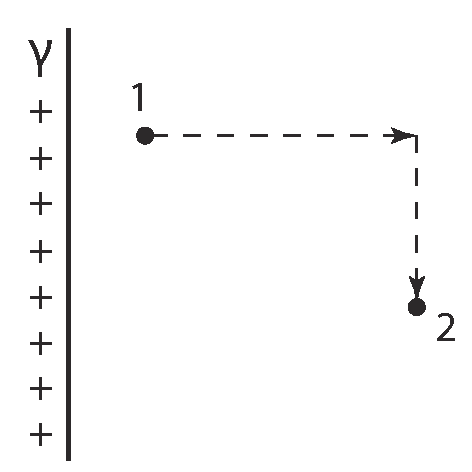
\includegraphics[width=.3\textwidth]{lec03/thread_field.pdf}
        \hfill
        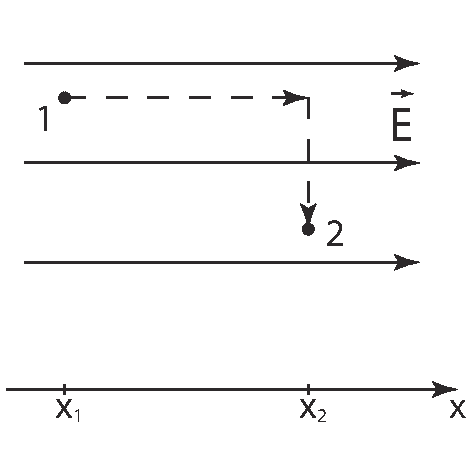
\includegraphics[width=.3\textwidth]{lec03/plane_field.pdf}
        \hfill
        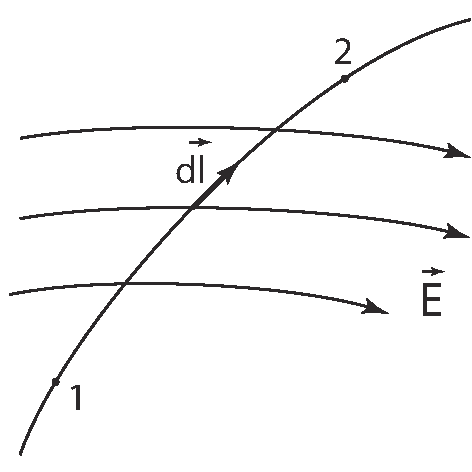
\includegraphics[width=.3\textwidth]{lec03/potential.pdf}
        \parbox[t]{.3\textwidth}{\caption{К вычислению потенциала поля заряженной нити}}
        \hfill
        \parbox[t]{.3\textwidth}{\caption{Разность потенциалов в однородном поле}}
        \hfill
        \parbox[t]{.3\textwidth}{\caption{Связь напряженности поля с его потенциалом}}
    \end{figure}

    \begin{example} % picture here or somewhere near
        Определить разность потенциалов между точками 1 и 2 в поле
        \( \vec{E} = \const \).
    \end{example}
    
    \begin{solution}
    Так как \( \Delta\varphi_{1 \to 2} \) не зависит от формы пути, то выбираем 
    путь так: \( 1 \to 2 = 1 \to 1’ + 1’ \to 2 \).
    \[
        \Delta\varphi_{1 \to 2} = \int\limits_1^{1’} \vec{E}\cdot\dd\vec{l} + 
        \int\limits_{1’}^2 \vec{E}\cdot\dd\vec{l} = E \Delta x = E(x_2 - x_1)
    \]
    \end{solution}

\section{Выражение поля \textbf{E} через заданное распределение потенциала}

    Формула (\ref{eq3:2}) даёт выражение \( \varphi (x, y, z) \) через заданное 
    поле \( \vec{E} (x, y, z) \).
    Поставим обратную задачу: как найти \( \vec{E} (x, y, z) \) через
    \( \varphi (x, y, z) \)?
    
    \begin{solution} % funky picture again.
    Выделим на кривой \( L \) в поле \( \vec{E} \) две близкие точки 1 и 2.
    \[
        \varphi_2 = \varphi_1 + \Delta\varphi \Rightarrow 
        \vec{E}\cdot\dd\vec{l} = \varphi_1 - \varphi_2 = -\dd\varphi = -
        \left(\partder{\varphi}{x}\dd x + \partder{\varphi}{y}\dd y + 
        \partder{\varphi}{z}\dd z\right) = -\nabla\varphi\cdot\dd\vec{l} \]
    
    Таким образом,
    \[
        \vec{E}\cdot\dd\vec{l} = -\nabla\varphi\cdot\dd\vec{l},
    \]
    но, так как \( \dd\vec{l} \) -- любой произвольный отрезок, то 
    \begin{equation}
        \label{eq3:3}
        \vec{E} = -\nabla\varphi
    \end{equation}
    А компоненты поля \( \vec{E} \) имеют следующий вид:
    \begin{align*}
        & E_{x} = -\partder{\varphi}{x},\\
        & E_{y} = -\partder{\varphi}{y},\\
        & E_{z} = -\partder{\varphi}{z}
    \end{align*}
    \end{solution}
    
\section{Эквипотенциальные поверхности}
    \begin{figure}[b!]
        \center
        \subfigure[Поле одноимённых зарядов]{
        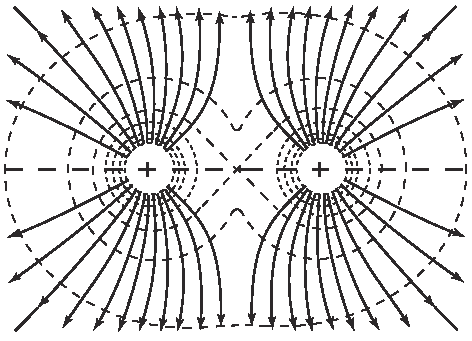
\includegraphics[width=0.47\textwidth]{lec03/equipot_same.pdf}}
        \subfigure[Поле разноимённых зарядов]{
        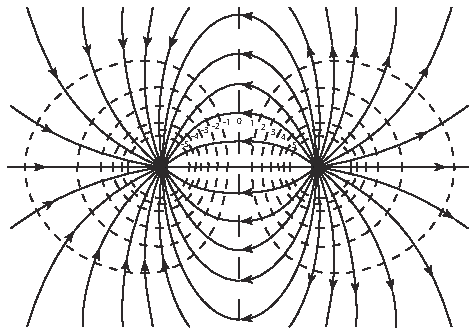
\includegraphics[width=0.47\textwidth]{lec03/equipot_different.pdf}}
        \caption{Эквипотенциали}
    \end{figure}

    \begin{definition}
        \textbf{Эквипотенциальные поверхности} -- это поверхности в пространстве, 
        на которых \( \varphi (x, y, z) = \const \), то есть эквипотенциали --  
        это поверхность уровня поля \( \varphi (x, y, z) \). 
    \end{definition}
    
    Так как \( \vec{E} = -\nabla\varphi \), и вектор \( \nabla\varphi \) 
    перпендикулярен к поверхности, на которой \( \varphi = \const \), то и 
    линии поля \( \vec{E} \) перпендикулярны к ней.

    Таким образом. семейства линий \( \vec{E} \) и эквипотенциальные 
    поверхности везде взаимно перпендикулярны.
    
\section{Электрический диполь}

    Электрический диполь -- это пара одинаковых зарядов \( +q \) и \( -q \), 
    разнесённых  на расстояние \( l \). Дипольный момент диполя равен 
    \[
        \vec{p} = q\vec{l},
    \]
    где \( l \) -- длина диполя.

    \begin{figure}[b]
        \center
        \subfigure[Молекула воды]{
        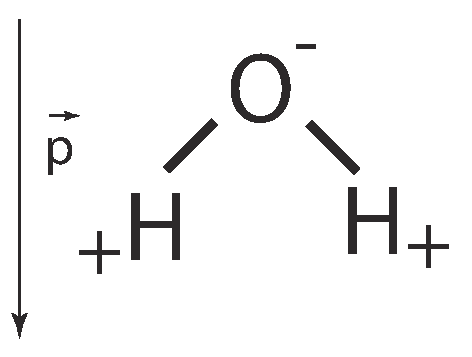
\includegraphics[width=0.18\textwidth]{lec03/water.pdf}}
        \subfigure[Молекула кислорода]{
        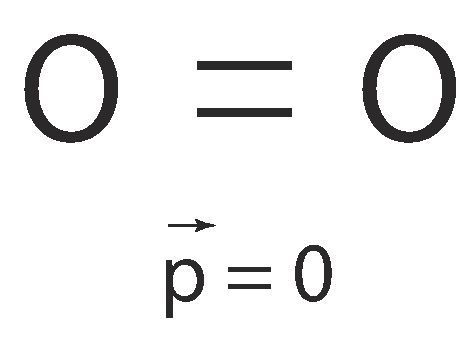
\includegraphics[width=0.18\textwidth]{lec03/oxygen.pdf}}
        \subfigure[Молекула озона]{
        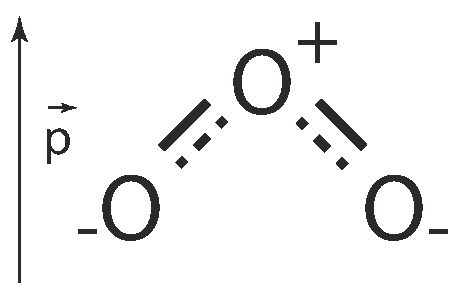
\includegraphics[width=0.18\textwidth]{lec03/ozone.pdf}}
        \subfigure[Молекула аммиака]{
        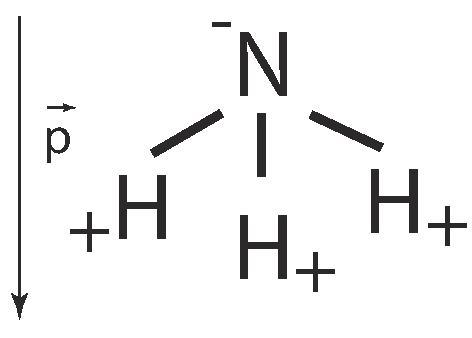
\includegraphics[width=0.18\textwidth]{lec03/ammonia.pdf}}
        \subfigure[Молекула метана]{
        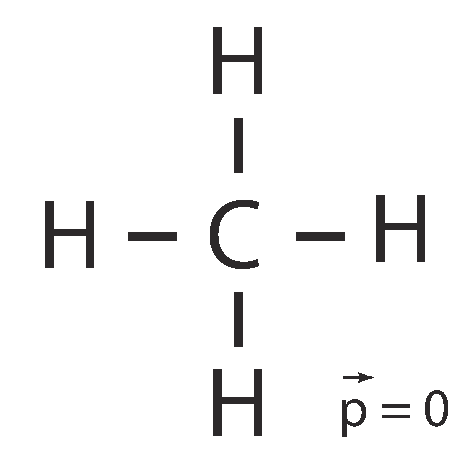
\includegraphics[width=0.18\textwidth]{lec03/methane.pdf}}
        \caption{Дипольные моменты молекул}
    \end{figure}   

    Зачастую, молекулы веществ являются диполями:   
    \begin{itemize}
        \item молекула воды \( H_2O \),
        \item молекула озона \( O_3 \),
        \item молекула аммиака \( NH_3 \).
    \end{itemize}

    Диполь называется точечным, если расстояние, с которого оценивается его 
    действие, много больше длины диполя.
    
\subsection{Потенциал и поле точечного диполя}

    \begin{figure}[b]
        \center
        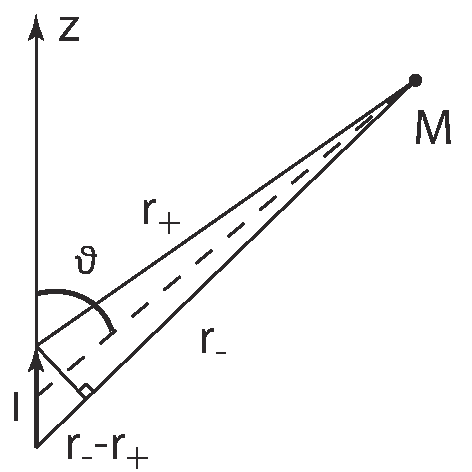
\includegraphics[width=.47\textwidth]{lec03/dipole_calculate.pdf}
        \hfill
        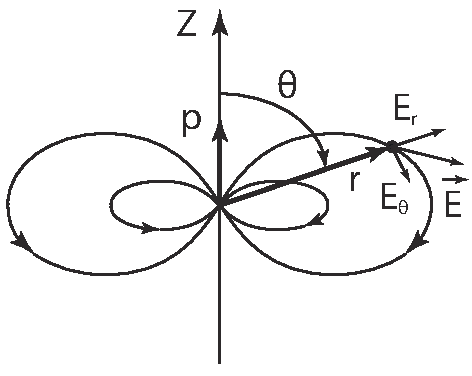
\includegraphics[width=.47\textwidth]{lec03/dipole_field.pdf}
        \parbox[t]{.47\textwidth}{\caption{Вычисление потенциала поля диполя}}
        \hfill
        \parbox[t]{.47\textwidth}{\caption{Поле диполя}}
    \end{figure}

    Вычислим потенциал и поле точечного диполя. Из свойства аддитивности
    потенциала следует:
    \[
        \varphi = \varphi_{+} + \varphi_{-}
    \]
    Или:
    \[
        \varphi = \frac{q}{4\pi\Ezero r_+} + \frac{-q}{4\pi\Ezero r_-} = 
        \frac{q}{4\pi\Ezero} \left(\frac{1}{r_+} - \frac{1}{r_-}\right) = 
        \frac{q}{4\pi\Ezero} \left(\frac{r_- - r_+}{r_-r_+}\right)
    \]
    
    Возьмём за \( r_-r_+  \approx r^2 \) -- расстояние от точки \( M \) до 
    диполя, а \( r_- - r_+ = l\cos\theta \).
    
    Таким образом, потенциал поля точечного диполя:
    \[
        \varphi = \frac{ql\cos{\theta}}{4\pi\varepsilon_0 r^2},
    \]
    где \( p = ql \) -- дипольный момент диполя,
    \( \theta = \widehat{\vec{p}\;\vec{r}} \) -- полярный угол.
    
    \begin{remark}
        У точечного заряда потенциал \( \varphi_{\textit{тз}} \sim r^{-1} \), а 
        у диполя \( \varphi_{\textit{диполя}} \sim r^{-2} \).
    \end{remark}
    
    Вычислим поле \( \vec{E} \) диполя. Так как \( \vec{E} = -\nabla\varphi \), 
    то в сферических координатах градиент \( \varphi \) равен:
    \begin{align*}
        & \nabla\varphi = \grad{\varphi} =
        \left\{ \frac{\partial\varphi}{\partial r}, 
        \frac{1}{r}\cdot\frac{\partial\varphi}{\partial\theta}, 
        \frac{1}{r\sin{\theta}}\cdot\frac{\partial\varphi}{\partial\psi} 
        \right\}, \\
        & E_r = -\frac{\partial}{\partial r}
        \left(\frac{p\cos{\theta}}{4\pi\varepsilon_0 r^2}\right) = 
        \frac{2p\cos{\theta}}{4\pi\varepsilon_0 r^3} = 
        \frac{p\cos{\theta}}{2\pi\varepsilon_0 r^3}, \\
        & E_{\theta} = -\frac{1}{r}\cdot\frac{\partial}{\partial\theta}
        \left(\frac{p\cos{\theta}}{4\pi\varepsilon_0 r^2}\right) = 
        \frac{p\sin{\theta}}{4\pi\varepsilon_0 r^3}.
    \end{align*}
    Таким образом,
    \[
        \vec{E}(r, \theta, \psi) = \frac{p}{4\pi\varepsilon_0 r^3}
        \{ 2\cos\theta, \sin\theta, 0 \}.
    \]
    А так как \( E_r \perp E_{\theta} \), то
    \begin{equation}
        E = \sqrt{ E_r^2 + E_{\theta}^2 } = 
        \frac{p}{4\pi\varepsilon_0 r^3}\cdot\sqrt{ 1 + 3\cos^2\theta }
    \end{equation}
    Работа этого поля по любому контуру всегда равна 0.

\subsection{Точечный диполь в однородном поле}
    \begin{figure}[b]
        \center
        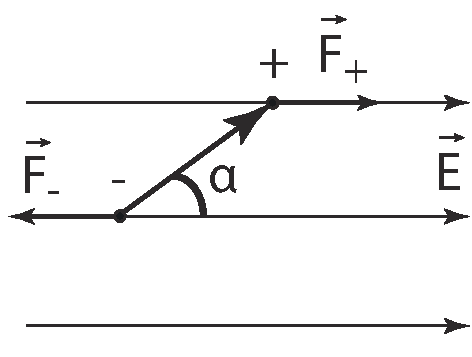
\includegraphics[width=.47\textwidth]{lec03/dipole_homogeneous.pdf}
        \hfill
        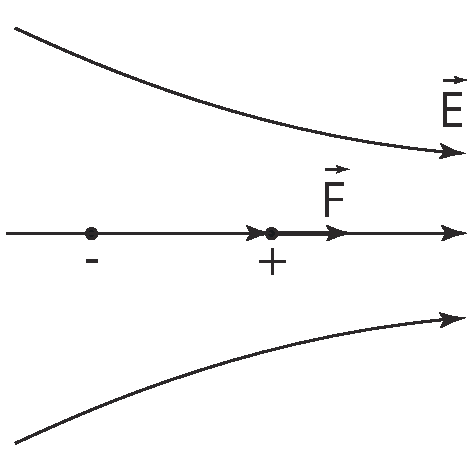
\includegraphics[width=.47\textwidth]{lec03/dipole_inhomogeneous.pdf}
        \parbox[t]{.47\textwidth}{\caption{Диполь в однородном поле}}
        \hfill
        \parbox[t]{.47\textwidth}{\caption{Диполь в неоднородном поле}}
    \end{figure}

    Пусть диполь помещён в однородное поле. Так как
    \( \vec{F_{-}} = -\vec{F_{+}} \), то \( \sum\vec{F} = 0 \). Однако, эта 
    пара сил создаёт момент \( M = lF_{+}\sin\alpha \) или
    \[
        \vec{M} = \vec{l}\times\vec{F_{+}} = q(\vec{l}\times\vec{E}) = 
        \vec{p}\times\vec{E}.
    \]
    
    Таким образом, в однородном поле действует момент:
    \begin{equation}
        \vec{M} = \vec{p}\times\vec{E}
    \end{equation}

    \subsection{Точечный диполь в неоднородном поле \textbf{E}}

    Момент сил, действующих на диполь, \( \vec{M} = \vec{p}\times\vec{E} \) 
    стремится повернуть диполь в ориентацию
    \( \vec{p} \uparrow\uparrow \vec{E} \). И если \( \vec{E} = \vec{E}(x,y,z)
    \ne \const \), то диполь втягивается в область более сильного поля.
    
    Вычислим энергию диполя в поле \( \vec{E} \).
    \( \sum\vec{F} = 0 \Rightarrow W_{\perp} = 0 \). Для поворота диполя в поле 
    \( \vec{E} \) необходимо совершить работу. Элементарная работа поворота:
    \[
        \dd A = M\dd\alpha = pE\sin\alpha \dd\alpha
    \]
    
    Тогда энергия диполя (ориентационная):
    \[
        W = A = \int pE\sin\alpha \dd\alpha = -pE\cos\alpha + C.
    \]
    Полагая, что при \( \vec{p} \perp \vec{E} \) энергия \( W = 0 \), получаем 
    \( C = 0 \). Таким образом,
    \begin{equation}
        W = -pE\cos\alpha = -\vec{p} \cdot \vec{E}.
    \end{equation}
    А так как в потенциальном поле \( \vec{F} = -\nabla W \), то в неоднородном 
    поле
    \[
        \vec{F} = \nabla(\vec{p}\cdot\vec{E}) = (\vec{p}\cdot\nabla)\vec{E}.
    \]
    
    В одномерном случае формула принимает вид
    \begin{equation}
        \vec{F}_x = p\frac{\partial E}{\partial x}
    \end{equation}
